\documentclass[12pt]{beamer}
\usepackage{mathptmx}
\title{Budgeting for a School Event}
\subtitle{How algebra helps plan costs and revenues}
\author{Presented by: Andrew Ralph}
\date{4/1/2026}

\usepackage{tikz}
\setbeamertemplate{background}{
    \begin{tikzpicture}[remember picture,overlay]
        \node[anchor=south east, xshift=5mm, yshift=5mm, opacity=0.3] at (current page.south east) {\small\textit{Courtesy of LaTeX}};
    \end{tikzpicture}
}

\usepackage{pgfplots}
\pgfplotsset{compat=1.18}

\begin{document}
\begin{frame}
\titlepage
\end{frame}
\begin{frame}{The Event}
    Every year, our school hosts a little fundraiser event that allows clubs
    to set up and try to raise money for their causes.
    This year, the event reached an all time high so we've asked each club who
    participated to share their accounting charts with us so we can
    analyze these amazing young minds. Of the 7 clubs that participated
    5 of them made a profit 2 broke even and 0 of them Lost money. 
    Lets take a look at the numbers and see how they did it.

\end{frame}
\begin{frame}{The Budget}
    We'll start with the budget, which is the amount of money that each club
    had to spend on their booth. Each club had a different budget, but they all 
    had to spend money on materials, decorations, and supplies. The budgets ranged 
    from $100 to $500, with an average of $300. 

    \begin{columns}
    \column{0.5\textwidth}
    Here's a breakdown of the budgets for each club

    \column{0.5\textwidth}
        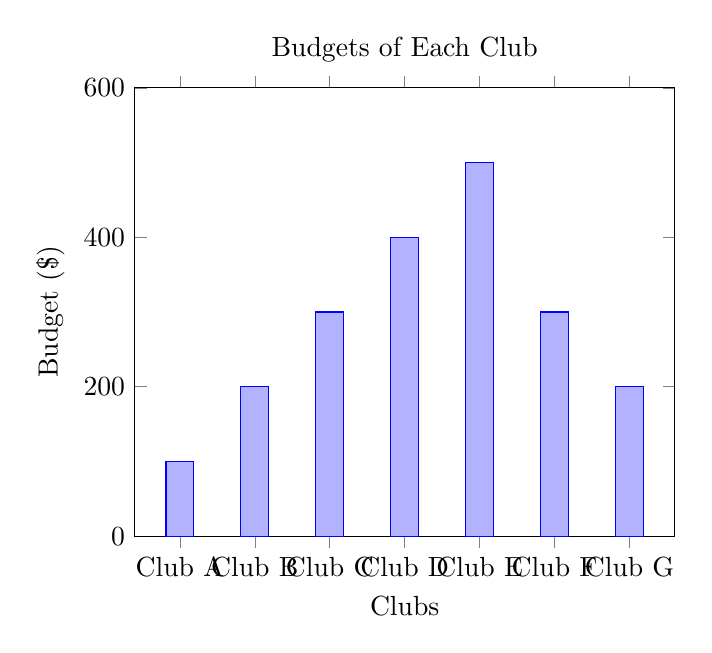
\begin{tikzpicture}
            \begin{axis}[
                ybar,
                symbolic x coords={Club A, Club B, Club C, Club D, Club E, Club F, Club G},
                xtick=data,
                ymin=0,
                ymax=600,
                ylabel={Budget (\$)},
                xlabel={Clubs},
                title={Budgets of Each Club}
            ]
            \addplot coordinates {(Club A, 100) (Club B, 200) (Club C, 300) (Club D, 400) (Club E, 500) (Club F, 300) (Club G, 200)};
            \end{axis}
        \end{tikzpicture}
    \end{columns}

\end{frame}
\begin{frame}{The Revenue}
    %content
\end{frame}
\begin{frame}{The Profit}
    %content
\end{frame}
\begin{frame}{The Break-Even Point}
    %content
\end{frame}
\begin{frame}{The Conclusion}
    %content
\end{frame}

\end{document}

